\section*{Appendix A: Details of models and datasets}

\begin{table}[h]
\centering
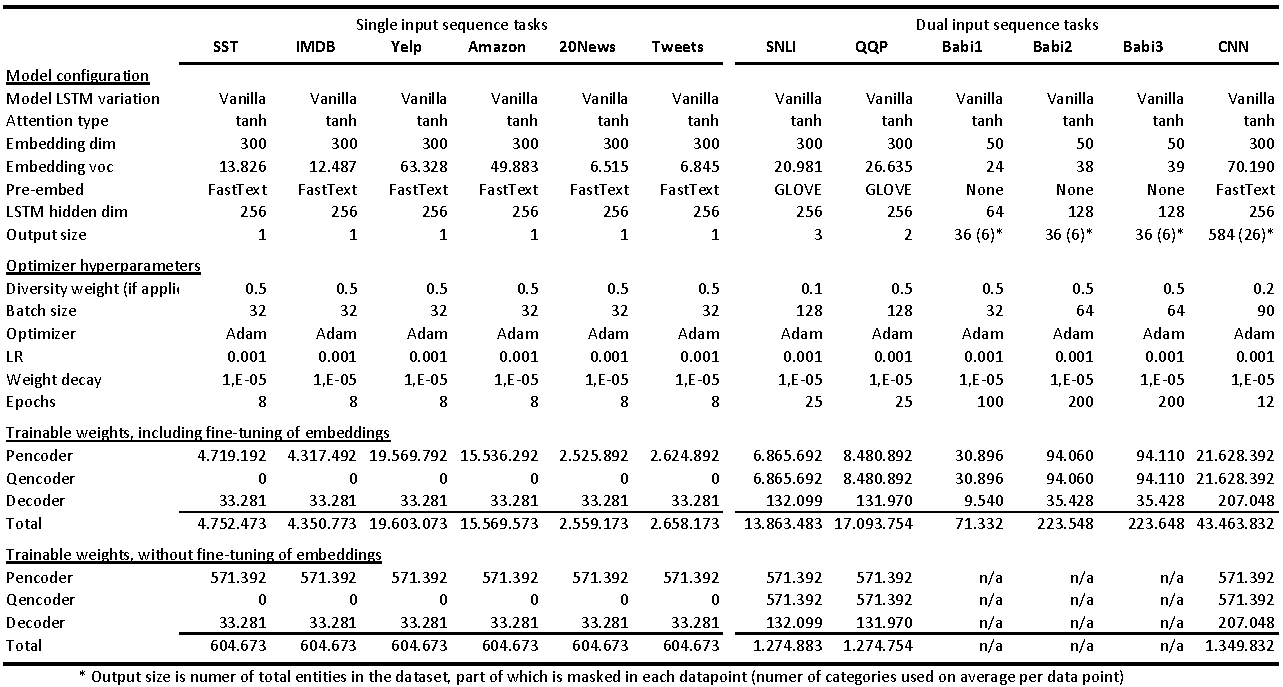
\includegraphics[width=\textwidth]{./figures/hyperparams.pdf}
\caption{Model- and hyperparameters for standard configurations per dataset}
\label{fig:hyperparams}
\end{table}

\begin{table}[h]
    \tiny
    \centering
    \begin{tabular}{llrrrcccr}
    \toprule
    & & \multicolumn{3}{c}{Number of datapoints} & \multicolumn{2}{c}{Avg seq. length (train)} & Avg.no.answer & Vocab. size\\
    Dataset & Description & train (\%pos) & dev (\%pos) & test (\%pos) & Document & Question & categories& (train, docs)\\
    \cmidrule(r){1-2} \cmidrule(r){3-5} \cmidrule(r){6-7} \cmidrule(r){8-8} \cmidrule(r){9-9}
    \multicolumn{5}{l}{\textbf{Single input sequence tasks}}\\
    \cmidrule(r){1-9}
        SST & Sentiment analysis  & 6,355 (52\%) & 821 (52\%) & 1,725 (50\%) & 21 & n/a & 2 & 13,703\\
        IMDB & Sentiment analysis  & 17,200 (50\%)& 4,297 (49\%) & 4,356 (50\%) & 182 & n/a & 2& 12,486\\
        Yelp & Sentiment analysis &345,285 (54\%)&4,790 (54\%)&26,866 (54\%)&74&n/a&2&63,304  \\
        Amazon$^*$&Sentiment analysis&1,528,080 (52\%)&4,456 (52\%)&331,774 (52\%)&57&n/a&2&49,881\\
        Anemia$^*$&Diagnosis prediction&-&-&-&-&-&-&-\\
        Diabetes$^*$&Diagnosis prediction&-&-&-&-&-&-&-\\
        20News & Topic classification & 1,145 (50\%)&278 (50\%) &357 (50\%)&119&n/a&2&5,904\\
        Tweets & Topic classification & 13,938 (12\%)&2,447 (13\%)&4,123 (12\%)&23&n/a&2&6,841 \\
    \cmidrule(r){1-2} \cmidrule(r){3-5} \cmidrule(r){6-7} \cmidrule(r){8-8} \cmidrule(r){9-9}    
        %\\
    \multicolumn{5}{l}{\textbf{Dual input sequence tasks}}\\ 
    \cmidrule(r){1-9}
        SNLI & Natural language inference & 549,367 & 9,842 & 9,824 & 16 & 10 & 3& 17,943\\
        QQP & Paraphrase detection & 327,460 (37\%)&36,384 (37\%)&40,430 (37\%) &15&15&2&26,172\\
        bAbI1 & Question answering & 8,500 & 1,500 & 1,000& 38&5& 6 & 20\\
        bAbI2 & Question answering&8,500&1,500&1,000&96&6&6&34\\
        bAbI3 & Question answering&8,500&1,500&1,000&309&9&6&34\\
        CNN & Question answering&380,298&3,924&3,198&764&14&26.1&>70,000\\
        \bottomrule
    \end{tabular}\\
    \tiny{$^*$ Replication could not be performed for these datasets due to either availability or memory size limits}\\
    \caption{Characteristics of the datasets}
    \label{tab:datasets}
\end{table}

\newpage

\section*{Appendix B: Full replication results}
\begin{figure}[h]
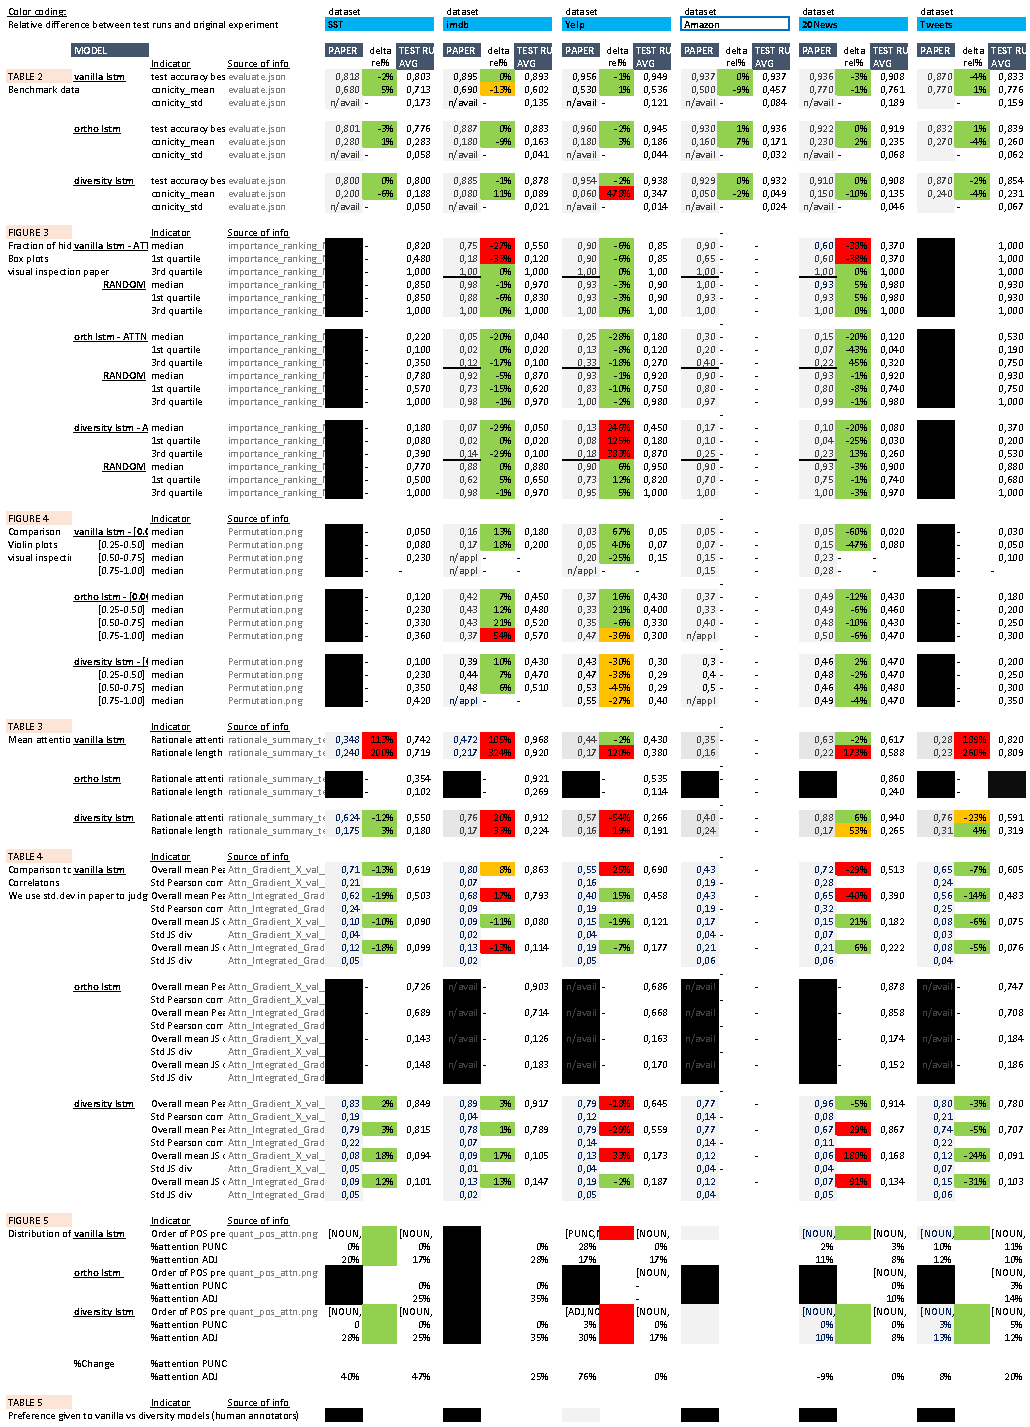
\includegraphics[scale=0.7, left]{./figures/repl_sst.pdf}
\caption{Replication results for single sequence tasks}
\label{fig:repr_test}
\end{figure}

\newpage

\begin{figure}[h]
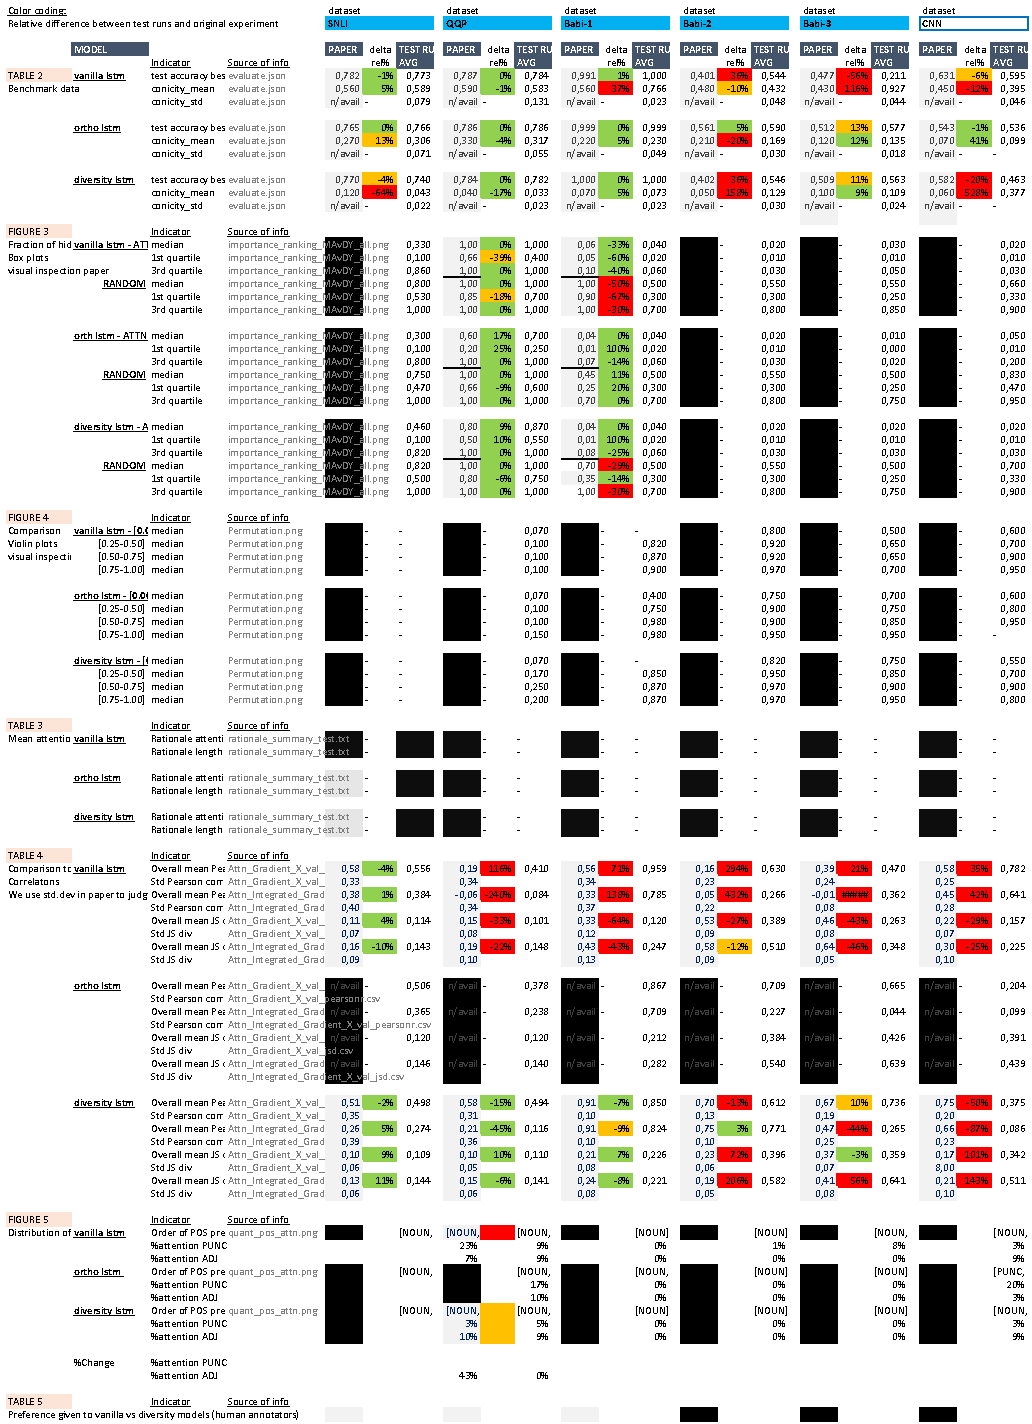
\includegraphics[scale=0.7, left]{./figures/repl_dst.pdf}
\caption{Replication results for dual sequence tasks}
\label{fig:repr_test2}
\end{figure}

\newpage

\section*{Appendix C: Results of BiLSTM extension}

\begin{figure}[h]
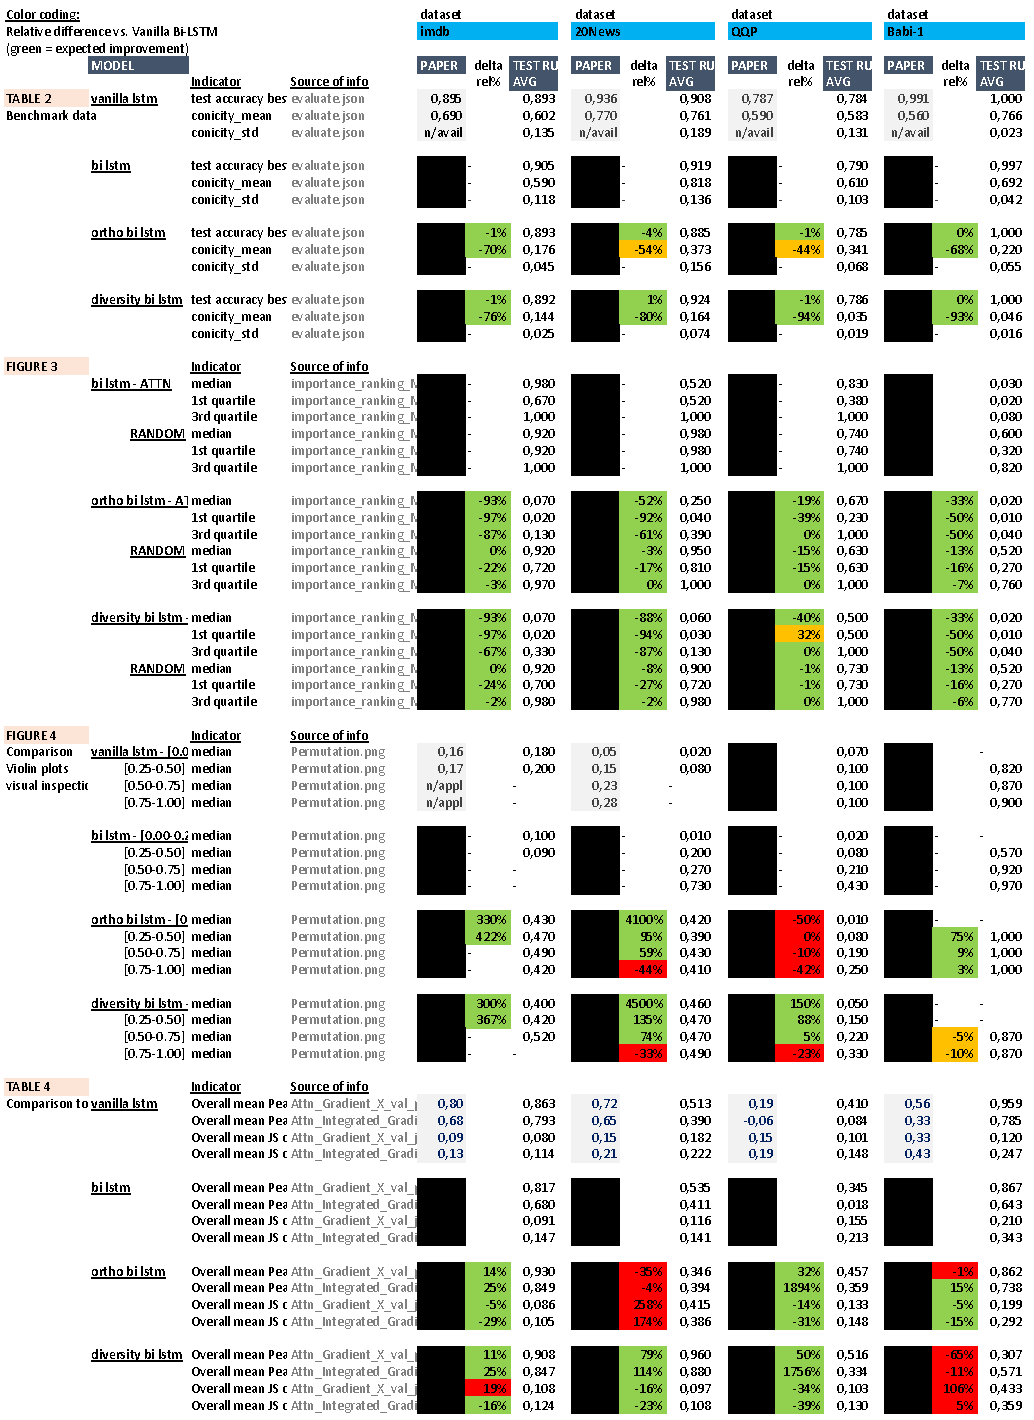
\includegraphics[scale=0.7, left]{./figures/bilstm_results.pdf}
\caption{Performance of BiLSTM on evaluation metrics}
\label{fig:results_bilstm}
\end{figure}

\newpage

\section*{Appendix D: Selected data examples and illustration of model behavior}

\begin{figure}[h]
\centering
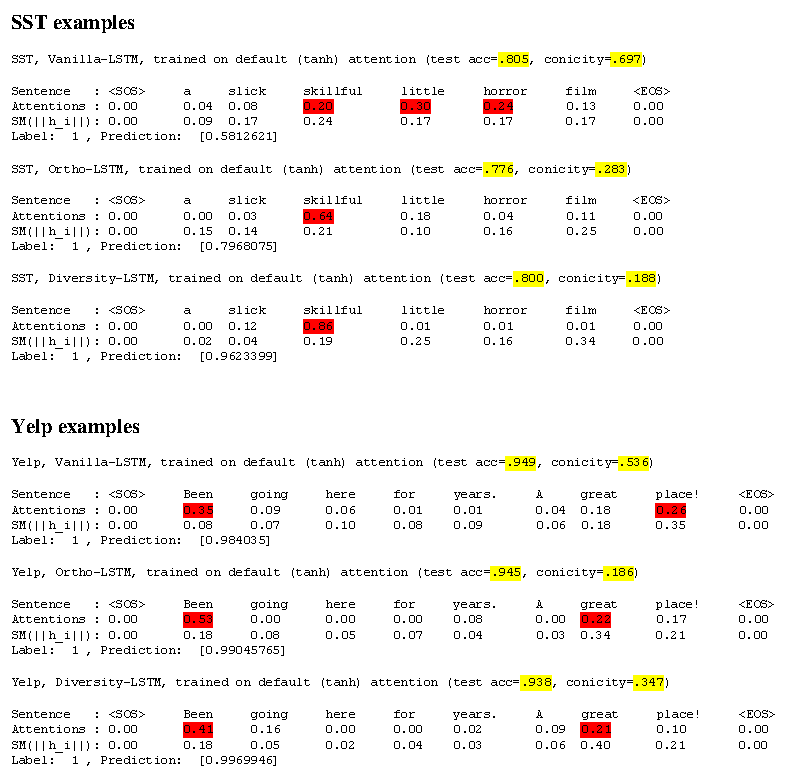
\includegraphics[width=1.0\textwidth,left]{./figures/BCexamples.pdf}
\caption{Examples of single input sequence tasks}
\label{fig:data_examples_1}
\end{figure}

\newpage

\begin{figure}[h]
\centering
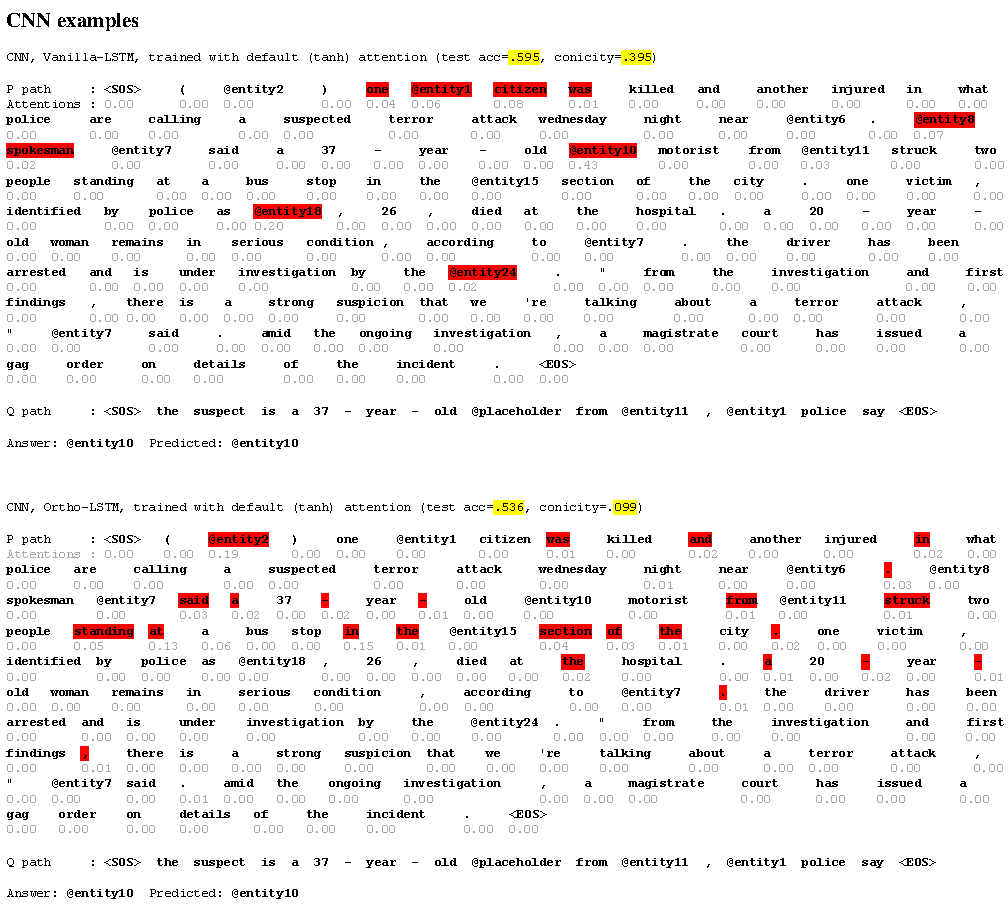
\includegraphics[width=1.0\textwidth,left]{./figures/QAexamples.pdf}
\caption{Examples of dual input sequence tasks}
\label{fig:data_examples_2}
\end{figure}